\documentclass[10pt]{beamer} 
\usetheme{cwc} 

\usepackage{amsmath,amssymb}
\usepackage{graphicx,acronym,setspace}
\usepackage[ruled]{algorithm2e}
\usepackage{subeqnarray,multirow,cite,array,color}

\acrodef{MSE}{mean squared error}
\acrodef{BC}{broadcast channel}
\acrodef{MC}{multi-cell}
\acrodef{BS}{base station}
\acrodef{MIMO}{multiple-input multiple-output}
\acrodef{SISO}{single-input single-output}
\acrodef{MU}{multi-user}
\acrodef{MU-MIMO}{\acl{MU} \acl{MIMO}}
\acrodef{OFDM}{orthogonal frequency division multiplexing}
\acrodef{WSRM}{weighted sum rate maximization}
\acrodef{QoS}{quality of service}
\acrodef{SCA}{successive convex approximation}
\acrodef{SNR}{signal-to-noise ratio}
\acrodef{MMSE}{minimum \acl{MSE}}
\acrodef{SIR}{signal-to-interference ratio}
\acrodef{SINR}{signal-to-interference-plus-noise ratio}
\acrodef{Q-WSRM}{queue \acl{WSRM}}
\acrodef{QM}{queue minimizing}
\acrodef{SRA}{spatial resource allocation}
\acrodef{JSFRA}{joint space-frequency resource allocation}
\acrodef{WMMSE}{weighted \acl{MMSE}}
\acrodef{KKT}{Karush-Kuhn-Tucker}
\acrodef{GP}{geometric programming}
\acrodef{SOC}{second-order cone}
\acrodef{BCDM}{block coordinate descent method}

\newcommand{\mbf}[1]{\mathbf{#1}}
\newcommand{\me}[1]{\( #1 \)}
\newcommand{\mc}[1]{\mathcal{#1}}
\newcommand{\fall}{\forall}
\newcommand{\set}[1]{\left \lbrace #1 \right \rbrace }
\newcommand{\mvec}[2]{\mathbf{#1}_{#2}}
\newcommand{\ith}[1]{{#1}^\mathrm{th}}
\newcommand{\pr}[1]{{#1}^\prime}
\newcommand{\mbfa}[1]{{\boldsymbol{#1}}}
\newcommand{\herm}{\mathrm{H}}
\newcommand{\sset}[1]{\left [ #1 \right ]}
\newcommand{\rfrac}[2]{{}^{#1}/{}_{#2}}
\newcommand{\eqspace}{\IEEEeqnarraynumspace}
\newcommand{\enoise}{\widetilde{N}_0}
\newcommand{\eqsub}{\IEEEyessubnumber}
\newcommand{\eqsubn}{\IEEEyesnumber \IEEEyessubnumber*}
\newcommand{\neqsub}{\IEEEnosubnumber}
\newcommand{\review}[1]{{\textcolor[rgb]{0 0 0.6}{#1}}}
\newcommand{\trace}{\mathrm{tr}}
\newcommand{\tran}{\mathrm{T}}
\newcommand{\R}[1]{\label{#1}\linelabel{#1}}
\newcommand{\lr}[1]{page~\pageref{#1}, line~\lineref{#1}}
\newcommand{\eqn}[1]{\(#1\)}
\newcommand{\mx}{\mbf{m}}
\newcommand{\my}{\mbf{w}}
\newcommand{\mz}{\mbfa{\gamma}}
\newcommand{\mxb}{{{\mbf{m}}}}
\newcommand{\myb}{{{\mbf{w}}}}
\newcommand{\iterate}[2]{{#1}^{(#2)}}
\newcommand{\iter}[3]{{#1}_{#2}^{(#3)}}
\newcommand{\ma}{\mbf{x}}
\acrodef{MSE}{mean squared error}
\acrodef{IBC}{interference broadcast channel}
\acrodef{MC}{multi-cell}
\acrodef{BS}{base station}
\acrodef{MIMO}{multiple-input multiple-output}
\acrodef{SISO}{single-input single-output}
\acrodef{MU}{multiple-users}
\acrodef{OFDM}{orthogonal frequency division multiplexing}
\acrodef{WSRM}{weighted sum rate maximization}
\acrodef{QoS}{quality of service}
\acrodef{SCA}{successive convex approximation}
\acrodef{SNR}{signal-to-noise ratio}
\acrodef{MMSE}{minimum \acl{MSE}}
\acrodef{SIR}{signal-to-interference ratio}
\acrodef{SINR}{signal-to-interference-plus-noise ratio}
\acrodef{Q-WSRM}{queue \acl{WSRM}}
\acrodef{QM}{queue minimizing}
\acrodef{SRA}{spatial resource allocation}
\acrodef{JSFRA}{joint space-frequency resource allocation}
\acrodef{WMMSE}{weighted \acl{MMSE}}
\acrodef{KKT}{Karush-Kuhn-Tucker}
\acrodef{GP}{geometric programming}
\acrodef{SOC}{second-order cone}
\acrodef{BCDM}{block coordinate descent method}
\acrodef{ADMM}{alternating directions method of multipliers}
\acrodef{PD}{primal decomposition}
\acrodef{DD}{dual decomposition}
\acrodef{FFR}{fractional frequency reuse}
\acrodef{DC}{difference of convex}
\acrodef{Q-WSRME}{\ac{Q-WSRM} extended}


\newcommand{\mbf}[1]{\mathbf{#1}}
\newcommand{\me}[1]{\( #1 \)}
\newcommand{\mc}[1]{\mathcal{#1}}
\newcommand{\fall}{\; \forall \;}
\newcommand{\set}[1]{\left \lbrace #1 \right \rbrace }
\newcommand{\mvec}[2]{\mathbf{#1}_{#2}}
\newcommand{\ith}[1]{{#1}^{\mathrm{th}}}

\graphicspath{{./../../ICASSP-2014/Figures/}}
\DeclareGraphicsExtensions{.eps}

\title{Queue Aware Precoder Design for Space Frequency Resource Allocation}
\author{{Ganesh Venkatraman, Antti T\"{o}lli, Le-Nam Tran and Markku Juntti} \\ \scriptsize{Email: \{gvenkatr, antti.tolli, le.nam.tran, markku.juntti\}@ee.oulu.fi}}

\begin{document}

\setstretch{1.3}

\begin{frame}
    \titlepage
\end{frame}

\begin{frame}{Outline}
    \tableofcontents
\end{frame}

\section{Introduction}

\begin{frame}{Introduction and Motivation}
\begin{itemize}
\item Complex algorithms are adopted to maximize the throughput to satisfy the data requirements of the higher layers
\item Available wireless resources are to be utilized efficiently to minimize the backlogged packets 
\item Spatial and Frequency resources are exploited to empty the packets waiting at the \acsp{BS}
\item In this work, we discuss the precoder design for the \acl{MU} \acs{MIMO}-\acs{OFDM} setup to minimize the number of queued packets 
\end{itemize}
\end{frame}

\section{System Model}

\begin{frame}{Symbols used}
\begin{itemize}
\item \acs{OFDM} system with \me{N} sub-channels and \me{N_B} \acsp{BS}, each equipped with \me{N_T} transmit antennas.
\item Let \me{K} users with \me{N_R} antennas each be present in the system
\item Users belonging to the \acs{BS} \me{b} is denoted by the set \me{\mc{U}_b \in \mc{U}}
\item Let \me{\mathcal{C} = \set{1,2,\dotsc,N}} be the set corresponding to the available sub-channels
\item The set of coordinating \acsp{BS} is represented by the set \me{\mc{B}}
\item Let \me{b_k \in \mathcal{B}} denotes the \ac{BS} serving the user \me{k}
\item Let \me{L} be the total available spatial streams for a user \me{k}, given by \me{\min (N_T,N_R)}
\end{itemize}
\end{frame}

\begin{frame}{System Model}
\begin{itemize}
\item The \me{\ith{l}} spatial signal received over the sub-channel \me{n} of the user \me{k} user is given by
\begin{multline*}\label{eqn-1}
y_{l,k,n} = \mvec{w}{l,k,n}^H \mvec{H}{b_k,k,n} \,\mvec{m}{l,k,n} d_{l,k,n} \\
 + \quad{} \mvec{w}{l,k,n}^H \sum_{i \in \mc{U} \backslash \set{k}} \mvec{H}{b_i,k,n} \sum_{j = 1}^L \mvec{m}{j,i,n}d_{j,i,n} + \tilde{n}_{l,k,n},
\end{multline*}
\item where \me{\mvec{m}{l,k,n}} and \me{\mvec{w}{l,k,n}} are the transmit and receive beamformer corresponding to the \me{\ith{l}} spatial stream over \me{\ith{n}} sub-channel for the user \me{k}
\end{itemize}
\end{frame}

\begin{frame}{System Model}
\begin{itemize}
\item \me{\mvec{H}{b_k,k,n} \in \mathbb{C}^{N_R \times N_T}} denotes the channel between the \acs{BS} \me{b_k} and the user \me{k}
\item \me{d_{l,k,n}} and \me{\tilde{n}_{l,k,n}} are the data and the equalized noise corresponding to the \me{\ith{l}} spatial stream of the user \me{k}
\item Now, the \acs{SINR} seen by the \me{\ith{l}} spatial stream over \me{\ith{n}} sub-channel for the user \me{k} is given by
\end{itemize}
\[ \gamma_{l,k,n} = \dfrac{\left |\mvec{w}{l,k,n}^H \, \mvec{H}{b_k,k,n} \, \mvec{m}{l,k,n} \right |^2}{N_0 + \sum_{(j,i) \neq (l,k)} |\mvec{w}{l,k,n}^H \mvec{H}{b_i,k,n} \mvec{m}{j,i,n} |^2}.\]
\end{frame}

\begin{frame}{Queueing Model}
\begin{itemize}
\item Each user is associated with the backlogged packets of size \me{Q_k} packets.
\item Queued packets \me{Q_k} of each user follows the dynamic equation at the \me{\ith{i}} instant as
\begin{equation}
Q_k(i) = \Big [ Q_k(i-1) - t_k(i-1) \Big ]^+ + \lambda_k(i),
\label{queue_dynamics}
\end{equation}
\item where \me{t_k = \sum_{n = 1}^N \, \sum_{l = 1}^L \, t_{l,k,n}} corresponds to the total transmitted packets of the user \me{k} in the previous \me{\ith{(i-1)}} instant
\item \me{\lambda_k} represents the arriving fresh packets for the user \me{k} at the \ac{BS} \me{b_k}
\end{itemize}
\end{frame}

\section{Problem Formulation}

\begin{frame}{Problem Formulation}
\begin{itemize}
\item Objective is to transmit the queued packets waiting at the \acsp{BS} to the corresponding users.
\item The available spatial and the frequency resources are to be utilized in an effective manner
\item In order to achieve this, precoders are to be designed with the similar objective
\item Precoders can perform scheduling of users by providing zero powers so as to eliminate from the resource elements
\end{itemize}
\end{frame}

\section{Proposed Solutions}

\subsection{\acs{Q-WSRM} Formulation}

\begin{frame}{Queue-Weighted Sum Rate Maximization (\acs{Q-WSRM})}
\begin{itemize}
\item \acs{Q-WSRM} formulation is the result of minimizing the conditional Lyapunov drift \footnote{Neely, Michael J. "Stochastic network optimization with application to communication and queueing systems." Synthesis Lectures on Communication Networks 3.1 (2010): 1-211.}
\item \acs{Q-WSRM} formulation is also called as back pressure algorithm, since it acts greedily in minimizing the backlogged packets at each instant
\[ \underset{t_{l,k,n}}{\text{minimize}} \quad \sum_{k \in \mc{U}} \left \lbrace Q_k(i)^2 - Q_k(i-1)^2 \right \rbrace, \]
\item where \me{Q_k} follows the dynamic Queue expression in \eqref{queue_dynamics} and \me{t_k = \sum_{n = 1}^N \, \sum_{l=1}^L \, t_{l,k,n}}
\end{itemize}
\end{frame}

\begin{frame}{Queue-Weighted Sum Rate Maximization (\acs{Q-WSRM})}
\begin{itemize}
\item Upon solving the Lyapunov drift expression, we obtain the \acs{Q-WSRM} formulation as
\end{itemize}
\begin{subequations}
\begin{align}
 \underset{t_{l,k,n}}{\text{maximize}} & \qquad \sum_{k \in \mc{U}} \; Q_k \left ( \alert{\sum_{n=1}^N} \, \sum_{l = 1}^L  t_{l,k,n} \right ) \\
& \qquad {\color{blue} \alert{\sum_{n=1}^N} \, \sum_{l = 1}^L  t_{l,k,n}  \leq \alert{Q_k} \; / \; Q_{k,n}}
\end{align}
\end{subequations}
\begin{itemize}
\item Performs better in the cell-edge scenario
\item Since each sub-channels are interference free, the queues are updated after designing the precoders at each sub-channels as
\end{itemize}
\begin{equation*}
Q_{k,n} = \max{\Big \lbrace Q_k - \sum_{j = 1}^{n-1} \, \sum_{l = 1}^{L} \, t_{l,k,j} ,0 \Big \rbrace }, \; \forall \; k \in \mathcal{U}
\end{equation*}
\end{frame}

\subsection{\acs{JSFRA} Formulation}

\begin{frame}{\acs{JSFRA} Formulation}
\begin{itemize}
\item Precoders are designed by a centralized controller, which is then used for the transmission by the \acsp{BS} in \me{\mc{B}}
\item The objective used to design the precoders is 
\[ {\color{blue} v_k = \left | Q_k - \sum_{n = 1}^N \sum_{l = 1}^{L} t_{l,k,n} \right |^q } \]
\item To generalize the objective, we use \me{\tilde{v}_k \triangleq a_k \, v_k}, where \me{a_k} is arbitrary weights used control the priorities
\item Exponent \me{q} plays different role based on the value it assumes
	\begin{itemize}
	\item \me{\ell_{q=1}} results in greedy allocation
	\item \me{\ell_{q=2}} ideal for the delay or buffer size limited scenarios
	\item \me{\ell_{q=\infty}} provides fair resource allocation
	\end{itemize}
\end{itemize}
\end{frame}

\begin{frame}{\acs{JSFRA} Formulation}
\begin{itemize}
\item Now, the precoder design problem is given as
\end{itemize}
\begin{subequations} \label{eqn-6}
\begin{align}
\underset{{t_{l,k,n},\mvec{M}{k,n},\mvec{W}{k,n}}}{\text{minimize}} & \hspace{0.25em} && \| \tilde{\mbf{v}} \|_q \label{eqn-obj} \\
\text{subject to} & \hspace{0.25em} && t_{l,k,n}\leq \log_2(1 + \gamma_{l,k,n}) \\
& \hspace{0.25em} && \alert{\gamma_{l,k,n} \leq \dfrac{\left |\mvec{w}{l,k,n}^H \, \mvec{H}{b_k,k,n} \, \mvec{m}{l,k,n} \right |}{\beta_{l,k,n}}^2\triangleq f(\tilde{\mbf{u}}_{l,k,n})},\label{eqn-6.2}\\
& \hspace{0.25em} && \beta_{l,k,n}  \geq  N_0 + \sum_{(j,i) \neq (l,k)} |\mvec{w}{l,k,n}^H \mvec{H}{b_i,k,n} \mvec{m}{j,i,n} |^2, \label{eqn-6.3} \\
& \hspace{0.25em} && \sum_{n = 1}^N \sum_{k \in \mathcal{U}_b} \text{tr} \, (\mvec{M}{k,n} \mvec{M}{k,n}^H) \leq P_{{\max}}, \fall b
\end{align}
\end{subequations}
\begin{itemize}
\item where \me{\tilde{\mbf{u}}_{l,k,n}  \triangleq \{\mvec{w}{l,k,n}^H, \mvec{H}{b_k,k,n}, \mvec{m}{l,k,n},\beta_{l,k,n}\}}
\end{itemize}
\end{frame}

\begin{frame}{\acs{JSFRA} Formulation}
\begin{itemize}
\item To maximize the received \acs{SINR}, \me{\mvec{W}{k,n}} are modeled with the \acs{MMSE} receivers
\item The \acs{JSFRA} formulation in \eqref{eqn-6} is nonconvex due to the constraint defined by \eqref{eqn-6.2} as
\me{\alert{\gamma_{l,k,n} \leq \dfrac{\left |\mvec{w}{l,k,n}^H \, \mvec{H}{b_k,k,n} \, \mvec{m}{l,k,n} \right |}{\beta_{l,k,n}}^2}}
\item In order to solve the problem in \eqref{eqn-6}, we use \ac{SCA} approach for the constraint defined by \eqref{eqn-6.2}
\item Let, \me{f(\tilde{\mbf{u}}_{l,k,n})=(p_{l,k,n}^2 + q_{l,k,n}^2)/\beta_{l,k,n}}, where
\end{itemize}
\begin{subeqnarray}
p_{l,k,n} &\triangleq& \Re \set{{\mvec{w}{l,k,n}^H \mvec{H}{b_k,k,n} \mvec{m}{l,k,n}}}, \\
q_{l,k,n} &\triangleq& \Im \set{{\mvec{w}{l,k,n}^H \mvec{H}{b_k,k,n} \mvec{m}{l,k,n}}}
\end{subeqnarray}
\end{frame}

\begin{frame}{\acs{JSFRA} Formulation}
\begin{itemize}
\item Now, the first order Taylor approximation is used for the function \me{f(\tilde{\mbf{u}}_{l,k,n})} around an arbitrary point \me{\tilde{\mbf{u}}_{l,k,n}^{(i-1)}}
\item With this approximation, the problem in \eqref{eqn-6} can be solved using the well known solvers for the optimal precoders and \me{\tilde{\mbf{u}}_{l,k,n}}
\item Once the optimal precoders \me{\mvec{M}{k,n}} are evaluated, \me{\mvec{W}{k,n}} are updated using the \acs{MMSE} receivers
\item The local point \me{\tilde{\mbf{u}}_{l,k,n}^{(i-1)}} is updated with the current optimal point \me{\tilde{\mbf{u}}_{l,k,n}^{(i)}}
\item With the updated precoders and \me{\tilde{\mbf{u}}_{l,k,n}^{(i)}}, optimization is carried out in an iterative manner until convergence
\end{itemize}
\end{frame}

\section{Simulation Results}

\subsection{SISO Example}

\begin{frame}{\acs{SISO} Example}
\begin{itemize}
\item Let us consider a simple example with \me{N_T = N_R = 1}, \me{N=3} sub-channels, and \me{K = 3} users, each having \me{Q_k = 6}
\item Rates allocated to each user by the two schemes are outlined as 
\end{itemize}
\begin{table}
\centering
\renewcommand{\arraystretch}{1.25} \scriptsize
\( \begin{array}{|*{10}{c|}}
\hline
\multirow{2}{*}{{k}} & \multicolumn{3}{c|}{{n = 1}} & \multicolumn{3}{c|}{{n = 2}} & \multicolumn{3}{c|}{{n = 3}} \\
\cline{2-10}
 & h_{k,1} & {a} & {b} & h_{k,2} & {a} & {b} & h_{k,3} & {a} & {b} \\
\hline
1 &  1.70 & 0 & 4.91 & 0.52 & 0 & 0 & 0.55 & 2.04 & 0 \\
2 &  0.39 & 0 & 0 & 1.41 & 4.39 & 4.39 & 1.02 & 0 & 0 \\
3 &  2.34 & 5.81 & 0 & 1.25 & 0 & 0 & 2.31 & 0 & 5.77 \\
\hline
\end{array} \)
\caption{Sub channel wise allocation for a scheduling instant}
\label{tbl-1}
\vspace{-0.35cm}
\end{table}
\begin{itemize}
\item \me{\zeta = 5.76} bits for \acs{Q-WSRM} and \me{\zeta = 2.93} bits for \acs{JSFRA} scheme, where \me{\zeta = \sum_{k = 1}^K \left [ \, Q_k - t_k \,\right ]^+}
\item \acs{Q-WSRM} scheme depends on the sub-channel permutation pattern
\end{itemize}
\end{frame}

\subsection{MIMO Example}

\begin{frame}{System Model - \me{\lbrace \, N_B,N_T,N,K,N_R \, \rbrace = \lbrace \, 2,4,5,8,1 \, \rbrace}}
\begin{figure}
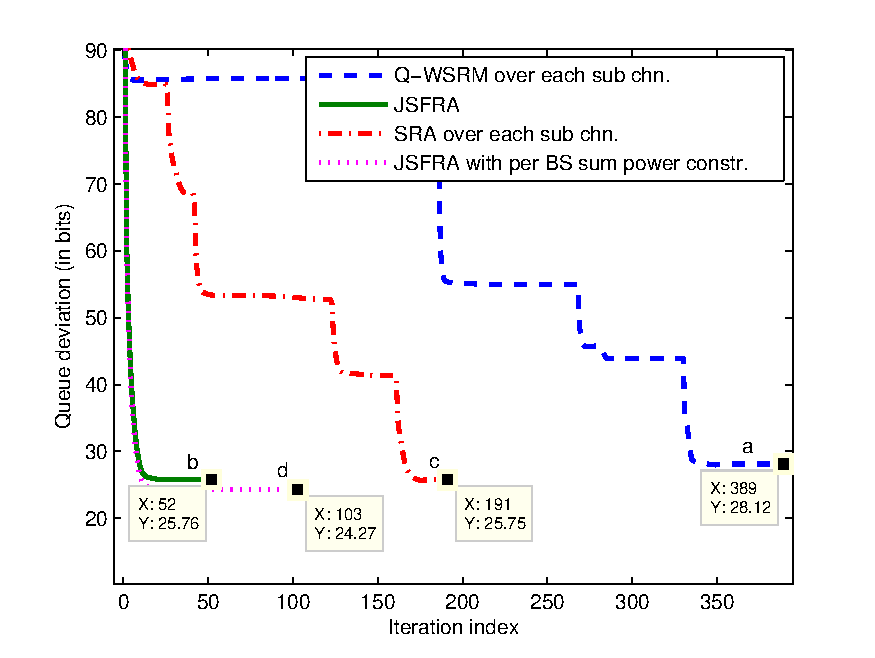
\includegraphics[width=0.8\textwidth]{qdeviation_4x1}
\end{figure}
\end{frame}

\begin{frame}{System Model - \me{\lbrace \, N_B,N_T,N,K,N_R \, \rbrace = \lbrace \, 2,4,5,8,2 \, \rbrace}}
\begin{figure}
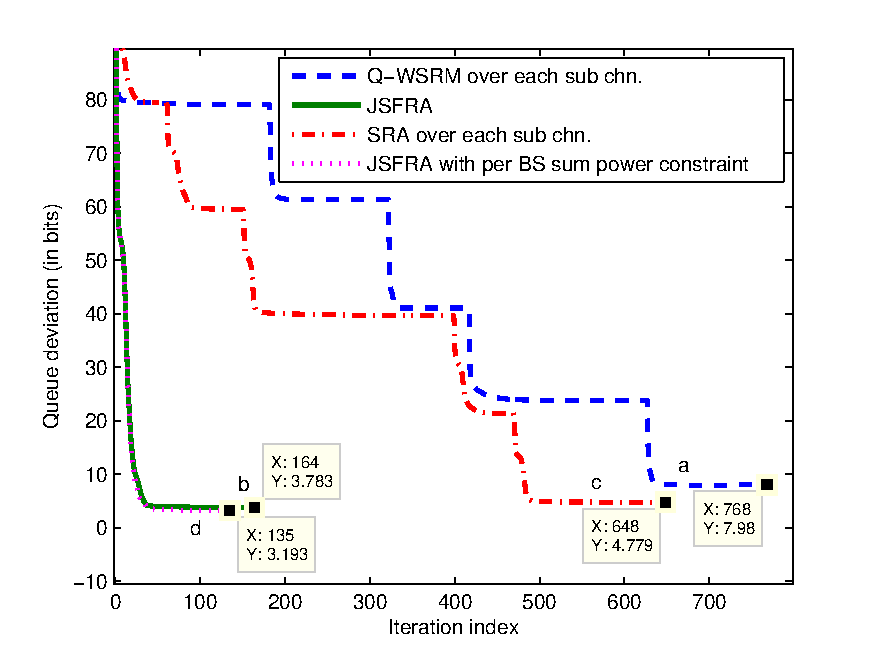
\includegraphics[width=0.8\textwidth]{qdeviation_4x2}
\end{figure}
\end{frame}

\begin{frame}{System Model - \me{\lbrace \, N_B,N_T,N,K,N_R \, \rbrace = \lbrace \, 2,4,3,6,1 \, \rbrace}}
\begin{figure}
\includegraphics[width=0.8\textwidth]{qdeviation_4x1_2}
\end{figure}
\end{frame}

\begin{frame}{System Model - \me{\lbrace \, N_B,N_T,N,K,N_R \, \rbrace = \lbrace \, 2,4,5,8,1 \, \rbrace}}
\begin{itemize}
\item Let the backlogged packets (bits) for each user be \me{Q_k = 12} bits
\item The resource allocation for different exponent \me{q}'s are given as
\end{itemize}
\begin{table}
\centering
\renewcommand{\arraystretch}{1.25} \scriptsize
\(\begin{array}{|c|*{8}{c}|c|}
\hline
{q} & \multicolumn{8}{c|}{\text{user indices}} & {\zeta} \\
\hline
{\ell_{1}} & 12.0 &  6.15 &  5.32 & 12.0 &  6.95 & 11.1 & 11.9 & 10.8 & 19.71 \\
{\ell_2} & 11.9 & 7.3 & 5.9 & 10.1 & 9.19 & 10.1 & 10.8 & 10.3 & 20.48 \\
{\ell_{\infty}} & 9.15 & 9.15 & 9.15 & 9.15 & 9.16 & 9.15 & 9.15 & 9.15 & 22.75 \\
\hline
\end{array}\)
\caption{Queue information for \me{N=5} sub-channels}
\label{tbl-3}
\vspace{-0.35cm}
\end{table}
\begin{itemize}
\item As seen from the table, for \me{q=1}, the resource are allocated in a greedy manner as compared to the \me{q=\infty}, which provides fair allocation of \me{\approx 9.15} bits each
\end{itemize}
\end{frame}

\section{Conclusions}

\begin{frame}{Conclusions}
\begin{itemize}
\item We discussed the problem of wireless resource allocation to minimize backlogged packets in an efficient way
\item The proposed approach uses \ac{SCA} method by using linear approximation for the nonconvex constraint
\item In future, we address the distributed approaches for the precoder design across each \acsp{BS} with minimal information exchange
\item An iterative algorithm for the \acs{JSFRA} scheme using \acs{MSE} reformulation will be addressed for the implementation purpose
\end{itemize}
\end{frame}


\begin{frame}
\begin{center}
{\color{blue}\Huge{Questions !}}
\end{center}
\end{frame}

\end{document}
